\documentclass{scrartcl}
\usepackage[utf8]{inputenc} % Umlaute werden erkannt
\usepackage{graphicx} % um png-Dateien einzubinden

\title{Übungsblatt 2}
\subtitle{Betriebssysteme und Systemsoftware, Sommersemester 2019}
\author{ \and Emma Ahrens, 371063}

\begin{document}
\maketitle

% Aufgabe 1
\section{Aufgabe}

% Aufgabe 2
\section{Aufgabe}

\subsection{}
Mit top kann man sich die Liste aller laufenden Prozesse anzeigen lassen. In der Liste sucht man sich die eindeutige PID heraus und beendet den jeweiligen Prozess mit kill X in der Kommandozeile, wo X die PID ist.

\subsection{}
Die Prozesse lassen sich mit ps -e anzeigen.

\subsection{}
Wenn man in der vierten Zeile char mit int ersetzt, dann terminiert das Programm.
Das liegt daran, dass ein unsigned char nur die Werte 0 bis 255 annehmen kann und wenn i = 255 gilt, wird ++i zu i = 0 ausgewertet. Ein unsigned int kann jedoch $2^{16}$ Werte annehmen, wobei $500 < 2^{16}$ gilt. Deshalb haben wir hier nicht das Problem eines Overflows. 

% Aufgabe 3
\section{Aufgabe}

\subsection{}
Siehe Figure 1.

\begin{figure}[ht]
	\centering
	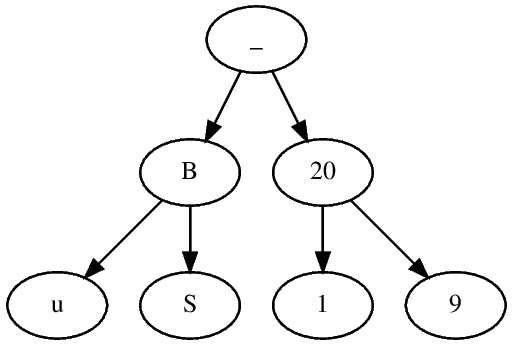
\includegraphics[width=0.33\textwidth]{Prozessbaum.png}
	\caption{Baum zur Aufgabe 3.1}
\end{figure}

\subsection{}
Da das Programm nur in den ersten Block geht, wenn fork() 0 ist, wird es in dem Block in der if-Bedingung immer fork() == 0 mit true auswerten. Also wird "u" ausgegeben und "S" kann nie ausgegeben werden.

% Aufgabe 4
\section{Aufgabe}

\end{document}
